\chapter{Bayesian Neural Networks}

\begin{wrapfigure}{r}{0.3\textwidth}
  \vspace{-40pt}
    \centering
    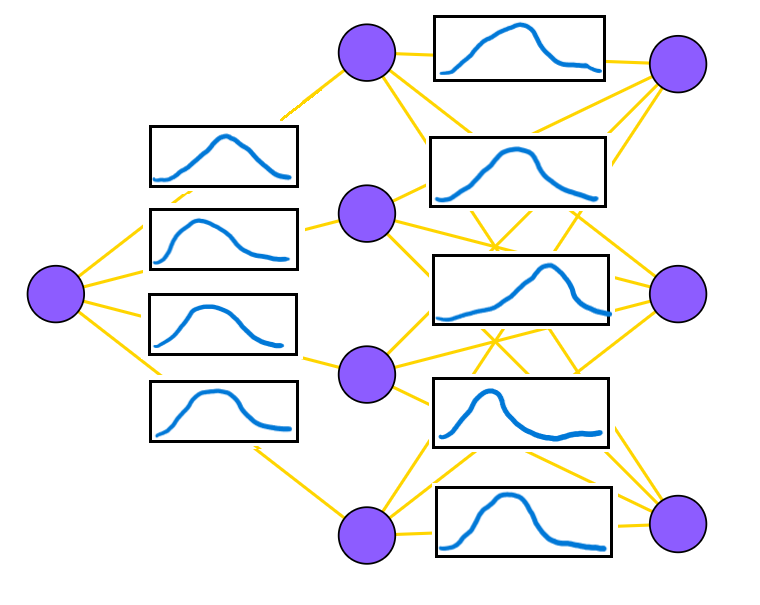
\includegraphics[width=.35\textwidth]{Figures/BNN_weightstoc.png}
    \caption{\footnotesize{A two-layer Bayesian Neural Network with parameters as distributions rather than strict point estimates.}}
  \label{BayesNet}
  \vspace{-10pt}
\end{wrapfigure}

 In the ``traditional'' non-Bayesian neural network framework, to train a neural network to minimize its error based on a single point estimate for each $w_i$, waged against a cost function, is to maximize the likelihood of the training data (i.e. finding weights $w_i$ that maximize $P(D_y|D_x,\theta)$ \cite{bishop1995} \cite{bishop1997bayesian}.  The drawback to an ANN is that the distribution of network parameters $\theta = (W,b)$ across the network is unknown. \cite{mullachery2018bayesian}  Without supplemental engineering, measurements of the model's uncertainty cannot be quantified.
 
 In Bayes, there are no point estimates. Instead, by use of Bayes’ Rule, an interval of potential parameters based on probabilities $p(\theta|D)$ is computed.  As such, the network can express uncertainty in its weights and biases through this posterior distribution. What's more is by the rudimentary feature of marginalization, uncertainty can be quantified for the predicted outputs $p(y|D)$ (for either $y$ as a regression prediction or classification label); even the very architecture of the model $p(A|D)$ can be expressed as a distribution \cite{bishop1995}.
 Bayesian Neural Networks (BNN) are able to learn from few data points and tell more of the story than their ANN counterparts.  Usually, fewer data points results in a network with higher prediction variability.  Even a network with very low variability, say one trained with many data points, comes readymade with a regularizer to ward overfitting. \cite{vladimirova2019understanding}
 

\section{Architecture}

Conceptually, the overall architecture remains when working with probabilistic (Bayesian) networks.  The selection of layers, neurons, activation and so on remain merely the same.  Indeed, more complex network types such as Convolutional Nets \cite{shridhar2019comprehensive} can be implemented and trained by a Bayesian approach.  The overall model does not have to be restricted by Bayes alone; it can be one layer or more in a network of otherwise point-estimate layers \cite{Jospin}.  The fundamental aspect of BNNs is their ability to be trained with a probabilistic approach; which means that the same network trained more than once will (very likely) never be tuned exactly the same way.


\subsection{Stochastic Modeling}


A researcher unsatisfied with a single point estimate for network output may consider simulating multiple networks, introducing a probabilistic effect to parameter tuning so as to not generate the same results. Stochastic neural networks, which use either stochastic activations \cite{yu2021simple} or stochastic weights, simulate a set of possible network outcomes $y$ with associated probability $p(y)$.  Aggregating independent predictors can lead to better predictions than single point estimates. \cite{Jospin}.  In comparing the predictions of multiple samples of $\hat{y}_i$, stochastic models better measure uncertainty.  A simple example is the regularization technique dropout \cite{goan2020bayesian} described earlier.  A neural network trained with dropout has a component randomness introduced by the selection of neurons removed from training.  If the dropout model was trained over and over again, it would contain slightly different parameter values reflective of this random noise.  There are other ways to introduce stochasticity into the model.  The Generative Adversarial Network \cite{ziyin2022stochastic} introduced in Chapter 1 implements a probabilistic component for its discriminator to identify.  %Variational Autoencoders (VAE) \cite{kingma2013auto} take generative models a step further by introducing Bayes as one part of many in their overall structure, but this is out of the scope of this thesis. 
Simply put, Bayesian neural networks are a special case of stochastic neural networks in which the ensemble of possible models is obtained using Bayesian inference. \cite{mackay1992practical}


\begin{comment}
For example in regression, the network could assume residual normality by introducing Gaussian noise in its data generation \cite{Jospin}.
That is, for parameterizing weights $w$:
\begin{gather*}
\theta \sim N(\mu,\sigma^2) \\
w \sim p(w|D,\theta)
\end{gather*}
This is the essence of how a BNN is a special case of a stochastic model.  The difference lies in that the stochastic element $\theta$ lies in the prior $p(\theta)$.
\end{comment}

\subsection{Selection of Priors}

There is no one-size-fits-all for machine learning models, and deep learning models only inflate this fact due to their enormous complexity \cite{Goodfellow-et-al-2016}.  Therefore, it can be interpreted \cite{Jospin} that prior assumptions are in place for all machine learning models, be it the optimization algorithm, regularizer, architecture, etc. These are implicit for non-Bayesian networks.  However, with Bayes, the prior assumptions are made explicit.  Yet, given the complexity of the network, it is not always intuitive how to select priors.  A beginner's start for a regression task is to select a normal prior $p(\theta) \sim N(\mu,\sigma^2)$.  This is analogous to the point-estimate weight decay regularization described in earlier chapters, but will be further discussed later in this chapter.  Despite this, there is no theoretical argument that makes a normal prior better than any other \cite{silvestro2020prior}; it simply has nice mathematical properties.


\subsection{Development}

Recall that $\theta$ represents the model weights and biases $(W,b)$.  $D$ is the training data from which the model learns, its inputs and outputs denoted with sibscripts $_x$ and $_y$.  Applying Bayes' Theorem, to determine the posterior distribution of $\theta$ requires selection of a prior and determination of the likelihood of the data:

$$
p(\theta|D) = \frac{p(D_{y}|D_{x},\theta)p(\theta)}{\int_\theta p(D_{y}|D_{x},\theta')p(\theta')d\theta'}
$$

The normalizing constant in the denominator is what has been seen before: the difficult (profoundly intractable for any informative BNN's) integral that requires estimation by Markov Chain Monte Carlo or variational inference.  If a normal prior is selected, the same calculation as that presented at the end of chapter 2 would apply to solve for $p(\theta|D)$; this just presents some notational simplicity.  Having displayed mathematical formulation previously, the majority of this chapter maintains probability notation to exemplify the concepts of probabilistic modeling.



\section{Inference}

Marginalization takes reign when determining the distribution of network predictions.  This means integrating out $\theta$ from the final model.  Given the posterior distribution of network parameters $p(\theta|D)$, the distribution of network predictions $p(y|x,D)$ is calculated as:
$$
p(y^*|x,D) = \int_\theta p(y^*|x,\theta)p(\theta|D)d\theta
$$

Usually in practice, due to the nature of stochastic networks, a collection of samples $\Theta$ is taken from $p(\theta|D)$ and $Y$ from $p(y|x,D)$ \cite{Jospin}. These samples are aggregated to measure uncertainty and generate an estimate $\hat{y}$.

\subsection{Description of Uncertainty}

A quick recap is in order for uncertainty definitions: \textit{Aleatoric} uncertainty is the level of uncertainty due to the noise or random variation of the data (i.e. error).  \textit{Epistemic} uncertainty is the measure of uncertainty a model has (i.e. variance).  BNN's allow for distinguishability between these types of uncertainty \cite{Jospin}.  $p(\theta|D)$ measures the epistemic uncertainty in the model.  With few data points, the model will express a high level variation in its choice of parameters rather than blindly returning a seemingly confident answer.  With more data points, this uncertainty reduces.

Aleatoric uncertainty is measured by $p(y|x,\theta)$, which is the conditional probability of the predicted output given the input predictors and model parameters.  This conditional probability is not isolated to Bayesian models; however, use of Bayes provides a means of inverting conditional probabilities when necessary \cite{Jospin}.


Let $y = \Phi_{\theta} (x) + \epsilon$ represent the value of $y$ from the approximated distribution of parameter estimates (with error $\epsilon$) given input $x$.
For regression tasks, usually models are averaged to summarize BNN predictions: 
$$
\hat{y} = \frac{1}{|\Theta|} \sum_{\theta_i} \Phi_{\theta_i}(x)
$$

Uncertainty is computed by the \textit{covariance matrix}:
$$
\Sigma_{y|x,D} = \frac{1}{|\Theta|-1} \sum_{\theta_i} (\Phi_{\theta_i}(x) - \hat{y}) (\Phi_{\theta_i}(x) - \hat{y})^\intercal
$$

For classification tasks, the estimator is the most likely class, that is $\hat{p} = max(p_i)$.  Uncertainty is measured by the relative probability of each class, summarized by the average.
$$
\hat{p} = \frac{1}{|\Theta|} \sum_{\theta_i} \Phi_{\theta_i}(x)
$$

It will be demonstrated in a later example that, using the full strength of the stochastic network, the underlying distribution of prediction values can be approximated and visualized. \cite{ziyin2022stochastic}


\subsection{Regularization with Priors}

%s\textit{(Inflate this section and give more evidence as to HOW BNN's prevent overfitting)}

ANN's built from a non-Bayesian approach aim to minimize a loss function.  As mentioned earlier, this is what maximizes the likelihood of the data.  Mathematically:
$$
min(E_D(D|\theta)) \equiv max(p(D_y|D_x,\theta)
$$
(For notational symmetry, $E_D(D|w,A)$ as was described in previous sections is now represented as $E_D(D|\theta)$)

Introducing prior assumptions, the Bayesian approach to finding the most likely point estimate from the posterior would look like:
$$
 max(p(D_y|D_x,\theta)p(\theta)
$$
Non-Bayesian networks introduce a regularizing term to prevent issues of overfitting.  Assumming loss is calculated as the negative log-likelihood, the non-Bayesian network with a term comprable to a prior would be represented by an additive term \cite{Jospin}.  That is:
$$
 max(p(D_y|D_x,\theta)p(\theta) \equiv min(E_D(D|\theta) + E_{\Theta}(\theta)
$$
Where $E_{\Theta}(\theta)$ is the new representation of $E_W(w|A)$ from earlier sections.  Therefore, it can be concluded that the prior distribution acts as a regularizing term for a BNN.  What's more is that the distributional assumptions of a prior overtly impact the regularization technique a BNN utilizes in comparison to its ANN counterpart \cite{vladimirova2019understanding}.  The selection of a Gaussian prior %, as was used to describe regularization at the end of Chapter 2, 
is the BNN parallel to a non-Bayesian ANN with weight decay.


%---Pathway to earthquakes_brnn file---
\subfile{earthquakes_brnn}







\section{Prospective Expansions}

As by design, this thesis has intended to further the reader's understanding of neural networks by use of the Bayesian paradigm.  It has outlined many preferable traits of BNNs and the functional suitability they have for revealing highly complex trends in data.
This section is devoted to the primary inspirations for further research on Bayesian Neural Networks, based either in theory or application, or both.

\subsection{Model Comparison}
As promised at the beginning of this chapter, Bayes can be applied to select an ideal capacity model \cite{bishop1997bayesian}.  Consider three networks of different capacities (for example, the the three networks from the Tohoku Earthquake MLP example, each with an additional hidden layer).  Now, suppose they are Bayesian networks represented as $A_1, A_2, A_3$ with the subscript representing the number of hidden layers.
$$
p(A|D) = \frac{p(D|A)p(A)}{p(D)}
$$
Without justification to prefer one model over the other, the prior $p(A)$ would be the same.  Therefore, the complexity of the model is contingent only upon the data likelihood under each model $p(D|A)$.  Different models can be compared; the model with the highest likelihood of the data has better evidence for its predictions. Below is an arbitrary representation of these networks.  More complex models fit a wider range of data \cite{bishop1997bayesian}, indicated by the wider curves.  However, these have less likelihood than simpler models for certain data sets; one of which is represented by the red line.

\begin{figure}[H]
    \centering
    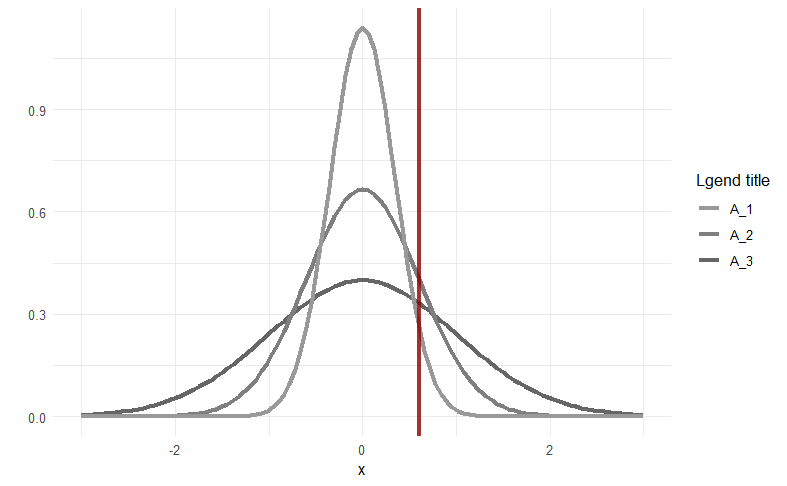
\includegraphics[width = .6\textwidth]{Figures/BNN_modelcheck.png}
    \caption{\footnotesize{Arbitrary representation of network generalizability, based on model complexity controlled by the number of hidden layers. Data within the central tendency of the red line may find the network with two hidden layers to be the most preferable}}
    \label{BNNmodelcheck}
\end{figure}

It would be interesting to compare specific architectures for the Tohoku Earthquake example, or any other appropriate example too.  Moving beyond, the application of Bayes to convolutional layers, specifically a comparison of probabilistic and deterministic models for high-level computer vision tasks, would be worth studying.


\subsection{Online Learning}
One can imagine scenarios in which the data is becoming available in real time, or even situations where a model is trained incrementally on data, as though it was fed through a hopper.  This makes especially interesting Bayesian techniques for online learning \cite{opper1999bayesian}, in which the BNN is trained in this way.  The Bayesian Updating rule would apply to cyclically recycle posteriors into priors in the presence of new data.  Further studies on this concept would be interesting to apply to practical application, such as in stock price fluctuation or weather prediction.

\subsection{BNN/ANN Regularizers}
It was noted several times that the assumptions of the prior distribution directly impact the BNN, specifically the recognizable regularization technique that its point-estimate correspondent would employ.  Literature \cite{vladimirova2019understanding} \cite{chiuso2016regularization} makes note of alternative priors and their coincidence with other regularization techniques (i.e. LASSO).  However, no publication exists based solely on the resemblance of probabilistic models with specific priors and their non-Bayesian counterparts.  It could be noteworthy to compare models built under each paradigm and demonstrate the level of engineering each would require as well as their predictive capabilities.


\begin{comment}
\section{Fitting a BNN}

Final run at the Tohoku Earthquake example that fits an \textit{ACTUAL} BNN with plenty of performance metrics displayed.


Each Subsection will be the main steps as shown in my R code.
\end{comment}